\documentclass{beamer}
% Use DS9 global theme
\usepackage{../../../../shared/templates/ds9_theme}

% Title page configuration
\title[Waves \& Sound]{PHYS11 CH: 5.5, 13, 14}
\subtitle{Oscillations, Waves, and Sound Physics}
\author[Mr. Gullo]{Mr. Gullo}
\date[Mar 2025]{March 24, 2025}
\institute{Physics Department}

% Begin document
\begin{document}

% Title page
\frame{\titlepage}

% Table of contents
\begin{frame}
\frametitle{Outline}
\tableofcontents
\end{frame}

%----------- SECTION: Introduction to Oscillations and Waves -----------
\section{Introduction to Oscillations and Waves}

\begin{frame}
\frametitle{Learning Objectives}
By the end of this presentation, you will be able to:
\begin{itemize}
\item Define and describe simple harmonic motion and its key parameters
\item Identify and explain different types of waves and their properties
\item Understand wave interactions including superposition and interference
\item Apply wave principles to sound phenomena
\item Solve problems involving wave speed, frequency, and wavelength
\item Explain resonance and calculate resonant frequencies
\end{itemize}
\end{frame}

\begin{frame}
\frametitle{Simple Harmonic Motion (SHM)}
\begin{columns}
\column{0.6\textwidth}
\begin{itemize}
\item An \textbf{oscillation} is a back and forth motion between two points
\item \textbf{Periodic motion} is a repetitious oscillation
\item \textbf{Period (T)}: Time for one complete oscillation
\item \textbf{Frequency (f)}: Number of oscillations per unit time
\begin{equation}
f = \frac{1}{T}
\end{equation}
\item An oscillation may create a \textbf{wave}, which propagates from its source
\end{itemize}

\column{0.4\textwidth}
\begin{figure}
    \centering
    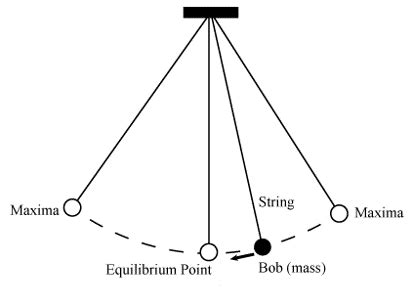
\includegraphics[width=1\linewidth]{phys11-waves-simple-harmonic-motion-spring.jpg}
\end{figure}
\end{columns}
\end{frame}

\begin{frame}
\frametitle{Hooke's Law and SHM}
The simplest oscillations are described by Hooke's Law:
\begin{equation}
F = -kx
\end{equation}
where:
\begin{itemize}
\item $F$ is the restoring force
\item $k$ is the spring constant
\item $x$ is the displacement from equilibrium
\end{itemize}

For a spring-mass system or simple pendulum (small angle):
\begin{align}
\text{Period in SHM: } T &= 2\pi \sqrt{\frac{m}{k}} \\
\text{Frequency in SHM: } f &= \frac{1}{2\pi}\sqrt{\frac{k}{m}} \\
\text{Period of pendulum: } T &= 2\pi \sqrt{\frac{L}{g}}
\end{align}
\end{frame}

%----------- SECTION: Wave Properties and Types -----------
\section{Wave Properties and Types}

\begin{frame}
\frametitle{Types of Waves}
\begin{block}{Definition}
A \textbf{wave} is a disturbance that moves from the point of creation and carries energy but not mass.
\end{block}

\begin{columns}
\column{0.5\textwidth}
\textbf{Based on medium requirement:}
\begin{itemize}
\item \textbf{Mechanical waves} must travel through a medium
\begin{itemize}
\item Sound waves
\item Water waves
\item Earthquake waves
\end{itemize}
\item \textbf{Non-mechanical waves} can travel through vacuum
\begin{itemize}
\item Light waves
\end{itemize}
\end{itemize}

\column{0.5\textwidth}
\textbf{Based on disturbance direction:}
\begin{itemize}
\item \textbf{Transverse waves}: Disturbance perpendicular to propagation
\item \textbf{Longitudinal waves}: Disturbance parallel to propagation
\end{itemize}

\textbf{Based on duration:}
\begin{itemize}
\item \textbf{Periodic waves}: Repeat for several cycles
\item \textbf{Pulse waves}: One or few crests, sudden disturbance
\end{itemize}
\end{columns}
\end{frame}

\begin{frame}
\frametitle{Wave Properties}
\begin{columns}
\column{0.6\textwidth}
\begin{itemize}
\item \textbf{Wavelength ($\lambda$)}: Distance between adjacent identical parts of the wave
\item \textbf{Amplitude}: Maximum displacement from equilibrium
\item \textbf{Period (T)}: Time for one complete wave cycle
\item \textbf{Frequency (f)}: Number of waves per unit time
\begin{equation}
f = \frac{1}{T}
\end{equation}
\item \textbf{Wave velocity ($v_w$)}: Speed at which wave moves
\begin{equation}
v_w = \frac{\lambda}{T} \text{ or } v_w = f\lambda
\end{equation}
\end{itemize}

\column{0.4\textwidth}
\begin{figure}
    \centering
    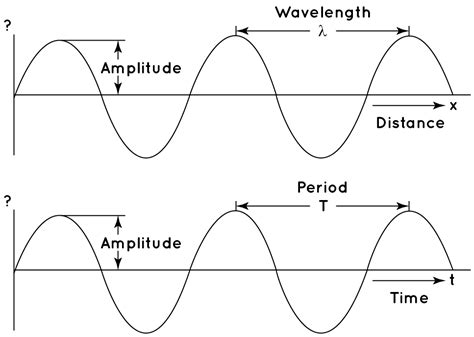
\includegraphics[width=1\linewidth]{phys11-waves-properties-wavelength-amplitude.jpg}
\end{figure}
\end{columns}
\end{frame}

\begin{frame}
\frametitle{Key Equations for Wave Motion}
\begin{block}{Wave Properties: Speed, Amplitude, Frequency, and Period}
\begin{align}
\text{Wave velocity: } v_w &= \frac{\lambda}{T} \text{ or } v_w = f\lambda \\
\text{Period: } T &= \frac{1}{f} \\
\text{Frequency: } f &= \frac{1}{T}
\end{align}
\end{block}

\begin{itemize}
\item In a given medium at a specific temperature (or density), the speed of a wave is the same for all frequencies and wavelengths
\item The relationship between wave velocity, frequency, and wavelength applies to all types of waves
\end{itemize}
\end{frame}

%----------- SECTION: Wave Interactions -----------
\section{Wave Interactions}

\begin{frame}
\frametitle{Superposition and Interference}
\begin{block}{Principle of Superposition}
When two or more waves overlap, the resultant displacement at any point is the algebraic sum of the displacements of the individual waves.
\end{block}

\begin{columns}
\column{0.5\textwidth}

\begin{figure}
    \centering
    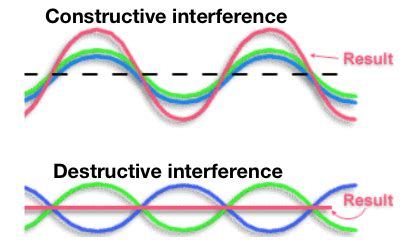
\includegraphics[width=1\linewidth]{phys11-waves-interference-constructive-destructive.jpg}
\end{figure}

\column{0.5\textwidth}
\textbf{Constructive Interference}
\begin{itemize}
\item Occurs when waves are in phase
\item Amplitudes add together
\item Results in a larger amplitude
\end{itemize}
\textbf{Destructive Interference}
\begin{itemize}
\item Occurs when waves are out of phase
\item Amplitudes subtract
\item Results in a smaller or zero amplitude
\end{itemize}
\end{columns}
\end{frame}

\begin{frame}
\frametitle{Standing Waves}
\begin{block}{Definition}
A \textbf{standing wave} is produced by the superposition of two identical waves traveling in opposite directions. It varies in amplitude but does not propagate.
\end{block}

\begin{itemize}
\item \textbf{Nodes}: Points where there is no motion
\item \textbf{Antinodes}: Locations of maximum amplitude
\end{itemize}

\begin{columns}
\column{0.6\textwidth}
\textbf{Other Wave Interactions:}
\begin{itemize}
\item \textbf{Reflection}: Wave changes direction
\item \textbf{Inversion}: Wave reflects from a fixed end
\item \textbf{Refraction}: Wave's path bends when passing between media with different densities
\end{itemize}

\column{0.4\textwidth}
\begin{figure}
    \centering
    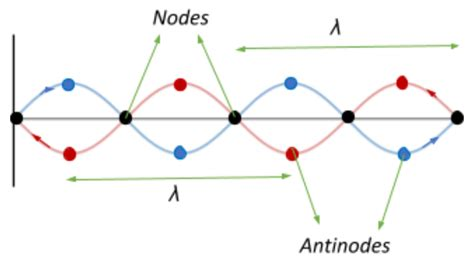
\includegraphics[width=1\linewidth]{phys11-waves-standing-wave-nodes.jpg}
\end{figure}
\end{columns}
\end{frame}

%----------- SECTION: Sound Waves -----------
\section{Sound Waves}

\begin{frame}
\frametitle{Sound Wave Characteristics}
\begin{block}{Definition}
\textbf{Sound} is a longitudinal mechanical wave created by a disturbance that is transmitted through a medium from its source outward.
\end{block}

\begin{itemize}
\item Sound waves require a medium to travel (cannot propagate in vacuum)
\item The relationship of speed, frequency, and wavelength:
\begin{equation}
v = f\lambda
\end{equation}
\item The speed of sound depends on the medium
\begin{itemize}
\item Air at 20°C: approximately 343 m/s
\item Water: approximately 1480 m/s
\item Steel: approximately 5960 m/s
\end{itemize}
\item In a given medium at specific temperature/density, the speed of sound is the same for all frequencies
\end{itemize}
\end{frame}

\begin{frame}
\frametitle{Sound Intensity and Sound Level}
\begin{columns}
\column{0.6\textwidth}
\begin{itemize}
\item \textbf{Sound intensity (I)}: Power per unit area
\begin{equation}
I = \frac{P}{A} = \frac{(\Delta p)^2}{2\rho v_w}
\end{equation}
where $\Delta p$ is pressure variation, $\rho$ is density, and $v_w$ is wave speed

\item \textbf{Sound intensity level} in decibels (dB):
\begin{equation}
\beta \text{ (dB)} = 10 \log_{10}\left(\frac{I}{I_0}\right)
\end{equation}
where $I_0 = 10^{-12}$ W/m² (threshold of hearing)
\end{itemize}

\column{0.4\textwidth}
Some typical sound levels:
\begin{itemize}
\item Whisper: 20 dB
\item Normal conversation: 60 dB
\item Busy traffic: 80 dB
\item Threshold of pain: 120 dB
\item Jet engine: 140 dB
\end{itemize}
\end{columns}
\end{frame}

\begin{frame}
\frametitle{Doppler Effect and Sonic Booms}
\begin{block}{Doppler Effect}
A shift in the observed frequency of a sound due to motion of either the source or the observer.
\end{block}

\begin{columns}
\column{0.6\textwidth}
\textbf{For a moving source:}
\begin{equation}
f_{obs} = f_s\left(\frac{v_w}{v_w \pm v_s}\right)
\end{equation}

\textbf{For a moving observer:}
\begin{equation}
f_{obs} = f_s\left(\frac{v_w \pm v_{obs}}{v_w}\right)
\end{equation}

Note: Use (+) when moving toward each other and (-) when moving apart

\column{0.4\textwidth}
\textbf{Sonic Boom}
\begin{itemize}
\item Occurs when an object moves faster than sound
\item Creates a shock wave
\item Result of constructive interference
\end{itemize}
\begin{figure}
    \centering
    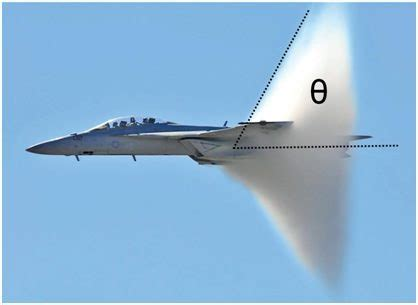
\includegraphics[width=0.5\linewidth]{phys11-waves-sonic-boom.jpg}
\end{figure}
\end{columns}
\end{frame}

%----------- SECTION: Sound Interference and Resonance -----------
\section{Sound Interference and Resonance}

\begin{frame}
\frametitle{Sound Interference Patterns}
\begin{itemize}
\item Sound waves can interfere constructively or destructively
\item \textbf{Beats}: Occur when waves of slightly different frequencies are superimposed
\begin{equation}
f_B = |f_1 - f_2|
\end{equation}
\item Beats are perceived as periodic variations in loudness
\item Used in tuning musical instruments
\end{itemize}
% \begin{figure}
%     \centering
%     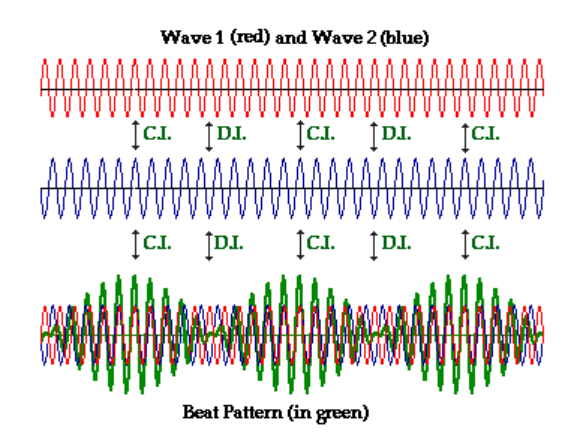
\includegraphics[width=0.5\linewidth]{BEAT.png}
% \end{figure}
% Note: BEAT.png image not found - needs to be replaced or recreated
\end{frame}

\begin{frame}
\frametitle{Resonance in Air Columns}
\begin{block}{Natural Frequency}
The frequency at which a system will oscillate if not affected by driving or damping forces.
\end{block}

\begin{block}{Resonance}
Occurs when a periodic force drives a harmonic oscillator at its natural frequency, resulting in maximum amplitude.
\end{block}

\begin{columns}
\column{0.5\textwidth}
\textbf{Tube closed at one end:}
\begin{equation}
f_n = n\frac{v}{4L}, \: n = 1,3,5...
\end{equation}
\begin{itemize}
\item Fundamental: $f_1 = \frac{v}{4L}$
\item Only odd harmonics
\end{itemize}

\column{0.5\textwidth}
\textbf{Tube open at both ends:}
\begin{equation}
f_n = n\frac{v}{2L}, \: n = 1,2,3...
\end{equation}
\begin{itemize}
\item Fundamental: $f_1 = \frac{v}{2L}$
\item All harmonics possible
\end{itemize}


\end{columns}
\end{frame}

\begin{frame}{}
    
\begin{figure}
    \centering
    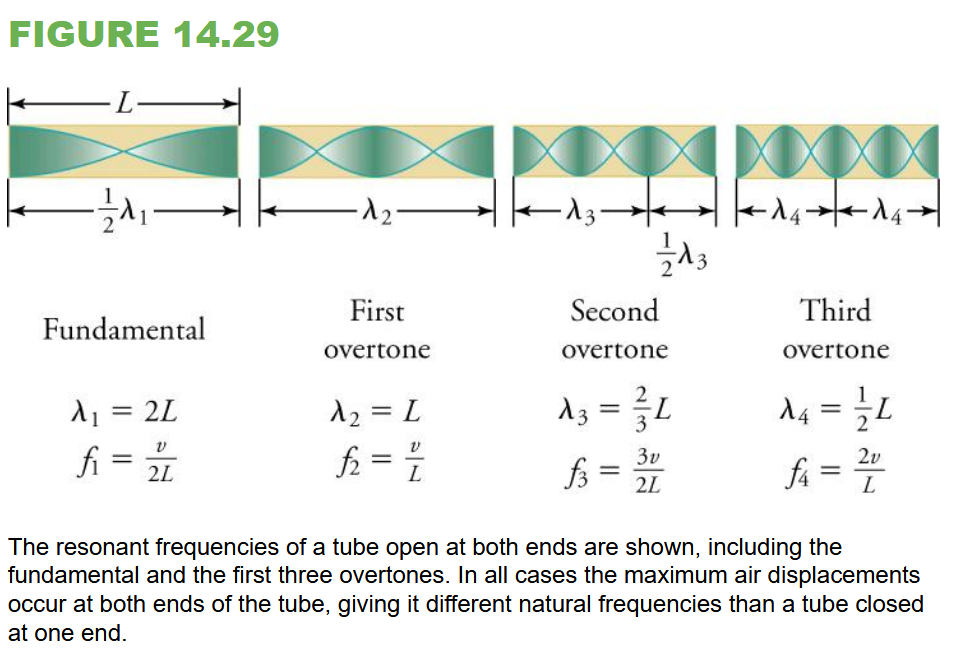
\includegraphics[width=1\linewidth]{phys11-waves-resonance-closed-tube.png}
\end{figure}

\end{frame}
\begin{frame}{}
    
\begin{figure}
    \centering
    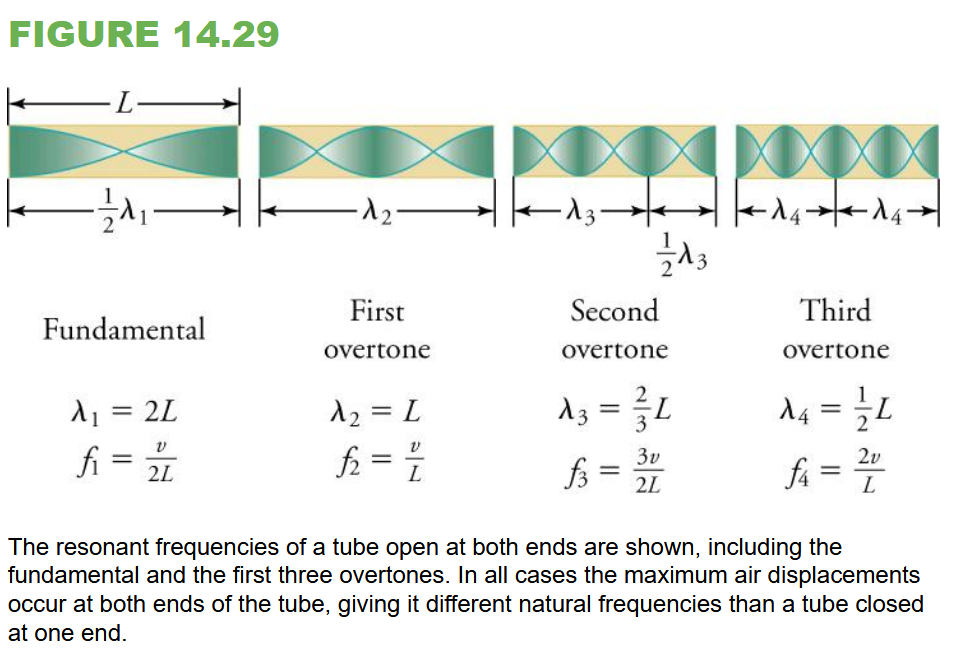
\includegraphics[width=1\linewidth]{phys11-waves-resonance-closed-tube.png}
\end{figure}
\end{frame}

%----------- SECTION: Problem-Solving Approach -----------
\section{Problem-Solving Approach}

\begin{frame}
\frametitle{"I do" - Wave Properties Example}
\begin{block}{Problem}
A wave has a frequency of 40 Hz and a wavelength of 0.5 m. Calculate the wave velocity.
\end{block}

\begin{block}{Solution}
Given:
\begin{itemize}
\item Frequency $f = 40 \text{ Hz}$
\item Wavelength $\lambda = 0.5 \text{ m}$
\end{itemize}

Using the wave velocity equation:
\begin{align}
v_w &= f\lambda \\
v_w &= 40 \text{ Hz} \times 0.5 \text{ m} \\
v_w &= 20 \text{ m/s}
\end{align}
\end{block}
\end{frame}

\begin{frame}
\frametitle{"We do" - Speed of Sound Example}
\begin{block}{Problem}
Sound travels at 343 m/s in air. If a sound wave has a frequency of 686 Hz, what is its wavelength?
\end{block}

\begin{block}{Partial Solution}
Given:
\begin{itemize}
\item Speed of sound $v = 343 \text{ m/s}$
\item Frequency $f = 686 \text{ Hz}$
\end{itemize}

Using the wave velocity equation:
\begin{align}
v &= f\lambda \\
343 \text{ m/s} &= 686 \text{ Hz} \times \lambda
\end{align}

Now, solve for $\lambda$...
\end{block}

\end{frame}

\begin{frame}
\frametitle{"You do" - Sound Resonance Example}
\begin{block}{Problem}
A tube open at both ends has a length of 0.85 m. If the speed of sound in air is 343 m/s, what are the frequencies of the fundamental and first two overtones?
\end{block}

\begin{block}{Approach}
1. Identify the type of resonator (open at both ends)
2. Recall the formula for resonant frequencies in an open tube
3. Calculate the fundamental frequency
4. Calculate the frequencies of the first two overtones
\end{block}

\textbf{Try it yourself!} We'll review the solution in a moment.
\end{frame}

\begin{frame}
\frametitle{"You do" - Sound Resonance Solution}
\begin{block}{Solution}
For a tube open at both ends:
\begin{equation}
f_n = n\frac{v}{2L}, \: n = 1,2,3...
\end{equation}

Given:
\begin{itemize}
\item Length $L = 0.85 \text{ m}$
\item Speed of sound $v = 343 \text{ m/s}$
\end{itemize}

Fundamental frequency ($n = 1$):
\begin{equation}
f_1 = \frac{343 \text{ m/s}}{2 \times 0.85 \text{ m}} = 201.8 \text{ Hz}
\end{equation}

First overtone ($n = 2$): $f_2 = 2f_1 = 403.5 \text{ Hz}$

Second overtone ($n = 3$): $f_3 = 3f_1 = 605.3 \text{ Hz}$
\end{block}
\end{frame}

%----------- SECTION: Summary -----------
\section{Summary}

\begin{frame}
\frametitle{Key Concepts Review}
\begin{columns}
\column{0.5\textwidth}
\textbf{Simple Harmonic Motion}
\begin{itemize}
\item Oscillations and periodic motion
\item Period and frequency relationship
\item Hooke's Law systems
\end{itemize}

\textbf{Waves}
\begin{itemize}
\item Types: mechanical/non-mechanical
\item Types: transverse/longitudinal
\item Properties: wavelength, amplitude, frequency
\item Speed-wavelength-frequency relationship
\end{itemize}

\column{0.5\textwidth}
\textbf{Wave Interactions}
\begin{itemize}
\item Superposition principle
\item Constructive/destructive interference
\item Standing waves, nodes, antinodes
\end{itemize}

\textbf{Sound}
\begin{itemize}
\item Longitudinal mechanical wave
\item Intensity and sound level
\item Doppler effect
\item Resonance and harmonics
\end{itemize}
\end{columns}
\end{frame}

\begin{frame}
\frametitle{Essential Equations}
\begin{columns}
\column{0.5\textwidth}
\textbf{Simple Harmonic Motion}
\begin{align}
F &= -kx \\
T &= 2\pi\sqrt{\frac{m}{k}} \\
T_{pendulum} &= 2\pi\sqrt{\frac{L}{g}}
\end{align}

\textbf{Wave Properties}
\begin{align}
v_w &= \frac{\lambda}{T} \text{ or } v_w = f\lambda \\
T &= \frac{1}{f}
\end{align}

\column{0.5\textwidth}
\textbf{Sound Intensity}
\begin{align}
I &= \frac{P}{A} = \frac{(\Delta p)^2}{2\rho v_w} \\
\beta \text{ (dB)} &= 10 \log_{10}\left(\frac{I}{I_0}\right)
\end{align}

\textbf{Resonance}
\begin{align}
f_B &= |f_1 - f_2| \\
f_n &= n\frac{v}{4L}, \: n = 1,3,5... \text{ (closed)} \\
f_n &= n\frac{v}{2L}, \: n = 1,2,3... \text{ (open)}
\end{align}
\end{columns}
\end{frame}

\begin{frame}
\frametitle{Connecting the Concepts}
\begin{itemize}
\item Simple harmonic motion creates oscillations
\item Oscillations can generate waves
\item Waves transport energy without transporting matter
\item Sound is a longitudinal mechanical wave
\item Wave properties (speed, frequency, wavelength) apply to all wave types
\item Wave interactions explain phenomena like resonance and interference
\item Understanding these principles helps explain everyday phenomena:
\begin{itemize}
\item Musical instruments
\item Hearing
\item Doppler radar
\item Medical ultrasound
\item Noise cancellation
\end{itemize}
\end{itemize}
\end{frame}

\begin{frame}
\frametitle{Thank You!}
\begin{center}
\Large Questions?
\end{center}
\end{frame}

\end{document}